\chapter{Introduction}
\label{introduction}

\begin{abstract}
Software testing is one of the essential and expensive tasks in software development. Hence, many approaches were introduced to automate different software testing tasks. Among these techniques, search-based test generation techniques have been vastly applied in real-world cases and showed promising results. These strategies apply metaheuristic search-based methods for generating tests according to various test criteria such as line coverage and branch coverage.

In this thesis, we introduce new search objectives and techniques using various knowledge carved from resources like source code, manually-written test cases, and execution logs. These novel search objectives and approaches (i) improve the state-of-the-art in search-based crash reproduction, (ii) present a new search-based approach to generate class-integration tests covering interactions between two given classes., and (iii) introduce two new search objectives for covering common/uncommon execution patterns observed during the software production.
\end{abstract}

\blfootnote{This chapter is partly based on \faFileTextO~\emph{P. Derakhshanfar. Well-informed Test Case Generation and Crash Reproduction, ICST'20 (Doctoral Symposium)}~\cite{derakhshanfar2020well}.
 }


\newpage
\dropcap{S}oftware testing is an indispensable part of software engineering, widely studied from various aspects by researchers in this field. As mentioned by Bertolino~\cite{bertolino2007software}, one of the biggest dreams in software testing research is 100\% automatic testing, and one of the research paths towards reaching this dream is the automation of test generation.

A survey by McMinn \cite{McMinn2004} shows that search-based software testing techniques are applicable to a vast range of automated software testing problems, including automated test generation. The application of metaheuristic search-based approaches for automating the process of software test generation has been an interesting research path in recent years. The approaches model the software testing goals, which should be achieved by manually-written test cases, into optimization problems and solve them using search algorithms. 

The approaches aim to produce tests for different levels of testing. For instance, many approaches are proposed for unit testing \cite{Fraser2011, braione2017tardis, braione2018sushi, prasetya2013t3} and system-level testing \cite{Arcuri2019, Holler2012, Padhye2019, beyene2012, coppit2005, godefroid2008}. Moreover, these approaches can be categorized into white-box \cite{Fraser2011, braione2017tardis, braione2018sushi, prasetya2013t3, Arcuri2019} and black-box \cite{Holler2012, Padhye2019, beyene2012, coppit2005, godefroid2008} testing techniques. 

The evaluations that were performed indicate the usefulness of the generated tests. More specifically, the generated tests can not only achieve high structural and mutation coverage~\cite{Panichella2018a, Fraser2014b}, but are also helpful for catching faults~\cite{Shamshiri2016} and debugging~\cite{Ceccato2015}. They have also been successfully deployed in industry~\cite{Alshahwan2018, almasi2017industrial}.

Most of these approaches aim at a general coverage criteria (\eg line and branch coverage). However,  generated tests with high structural coverage are not always successful at detecting faults. Gay \etal \cite{gay2015risks} have shown that these types of coverage criteria are poor indicators for failure detection and mutation score in some cases. As an example, a test case can cover a statement without passing failure revealing data. In this case, we have the coverage, but the fault will remain undetected without the adequate test oracle.
Moreover, Shamshiri \etal \cite{Shamshiri2016} reported that the tests generated by \evosuite, which is one of the better automatic unit test generation tools, are only successful in exposing about 50\% of industrial faults despite the high structural coverage scores. 

Furthermore, search-based test generation for specific problems has a lot of open challenges. Among them, fitness functions defined for search-based test generation suffer from a lack of guidance and underuse contextual information.  
In particular, Salahirad \etal \cite{Salahirad2019} indicated that the strongest fitness function (branch coverage) has about 25\% likelihood of fault detection.
As an outcome, they suggest using classical branch and line coverage as primary objectives and using other objectives that aid to trigger the faults as secondary objectives.

\begin{framed}
In this thesis, we go beyond classical search objectives based on structural coverage. In particular, we investigate how information collected from different sources (\ie source code, manually-written tests, \etc) can help to design and reinforce search objectives. In doing so, we hypothesize that we can exercise specific behaviors, and thus trigger specific kinds of faults.
\end{framed}

First, we focus on one of the instances of test generation for specific software behaviors: \textbf{search-based crash reproduction}. These crash reproduction approaches~\cite{Soltani2018a, BPT17concrash, Chen2015, Nayrolles2017, Rossler2013, Xuan2015} accept a crash as input and generate a test that reproduces this given crash. Our studies on crash reproduction focus on leveraging the collected contextual information to improve the effectiveness (\ie the number of reproduced crashes and how often they can be reproduced) and efficiency (\ie the time required to reproduce a crash) of the search process, trying to reproduce the given crash.

Second, we concentrate on generating tests for \textbf{exercising integration points between two classes}. We consider the execution of different scenarios in the interaction between two coupled classes as test objectives for the test generation process. We introduce a new test criterion for class integration testing, which is suitable for defining search objectives. Then, we design a search-based test generation algorithm according to this newly defined criterion. We investigate if this algorithm can reveal integration level faults which are not detectable with search-based unit testing.

Finally, we investigate a novel search objective for search-based unit testing that covers the \textbf{common and uncommon execution patterns}. To detect the common and uncommon patterns, we monitor the execution patterns during the operation of the software.

\section{Background \& Context}
This section presents an overview of search-based software test generation and automated crash reproduction and how they are connected to this thesis.

\subsection{Search-based Sofrware Test Generation}

McMinn~\cite{McMinn2004} defined search-based software testing (SBST) as \textit{``using a meta-heuristic optimizing search technique, such as a genetic algorithm, to automate or partially automate a testing task"}.
Within this realm, test data generation at different testing levels (such as \textit{unit testing}, \textit{integration testing}, \etc) has been actively investigated~\cite{McMinn2004}. This section 
provides an overview of earlier work in this area.

\paragraph{Search-based approaches for unit testing.}
SBST algorithms have been extensively used for unit test generation. Previous studies confirmed that thus generated tests achieve a high code coverage~\cite{Panichella2018a, Campos2018}, real-bug detection~\cite{almasi2017industrial}, and debugging cost reduction~\cite{soltani2017, Panichella2016}, complementing manually-written tests.

From McMinn's \cite{McMinn2004} survey about search-based test data generation, we observe that most of the current approaches rely on the control flow graph (CFG) to abstract the source code and represent possible execution flows. The $CFG_m=(N_m,E_m)$ represents a method\footnote{Or function in procedural programming languages.} $m$ as a directed graph of \textbf{basic blocks} of code (the nodes $N_m$), while $E_m$ is the set of the control flow edges. An edge connects a basic block $n_1$ to another one $n_2$ if the control may flow from the last statement of $n_1$ to the first statement of $n_2$. 

Listing~\ref{list:ClassA} presents the source code of \texttt{Person}, a class representing a person and her transportation habits. A \texttt{Person} can drive home (lines 4-10), or add energy to her car (lines 12-18). The right-hand side of Figure~\ref{fig:CCFG} presents the CFG of two of Person's methods, with the labels of the nodes representing the line numbers in the code. Since method \texttt{driveToHome} calls method \texttt{addEnergy}, \texttt{node 6} is transformed to two nodes, which are connected to the entry and exit point of the called method. This transformation is explained in the last paragraph of this section.  

\begin{lstlisting}[frame=tb,
    caption={Class \texttt{Person}},
    label=list:ClassA,
    language=java,
    captionpos=t,
    numbers=left,
    belowskip=-2.5em,
    float=t,
    firstnumber=1]
class Person{
    private Car car = new Car();
    protected boolean lazy = false;
    public void driveToHome(){
        if (car.fuelAmount < 100) {
            addEnergy();
        } else {
            car.drive();
        }   
    }

    protected void addEnergy(){
        if (this.lazy) {
            takeBus();
        } else {
            car.refuel();
        }
    }   
    }
  \end{lstlisting}

  \begin{figure}[t]
    \centering
	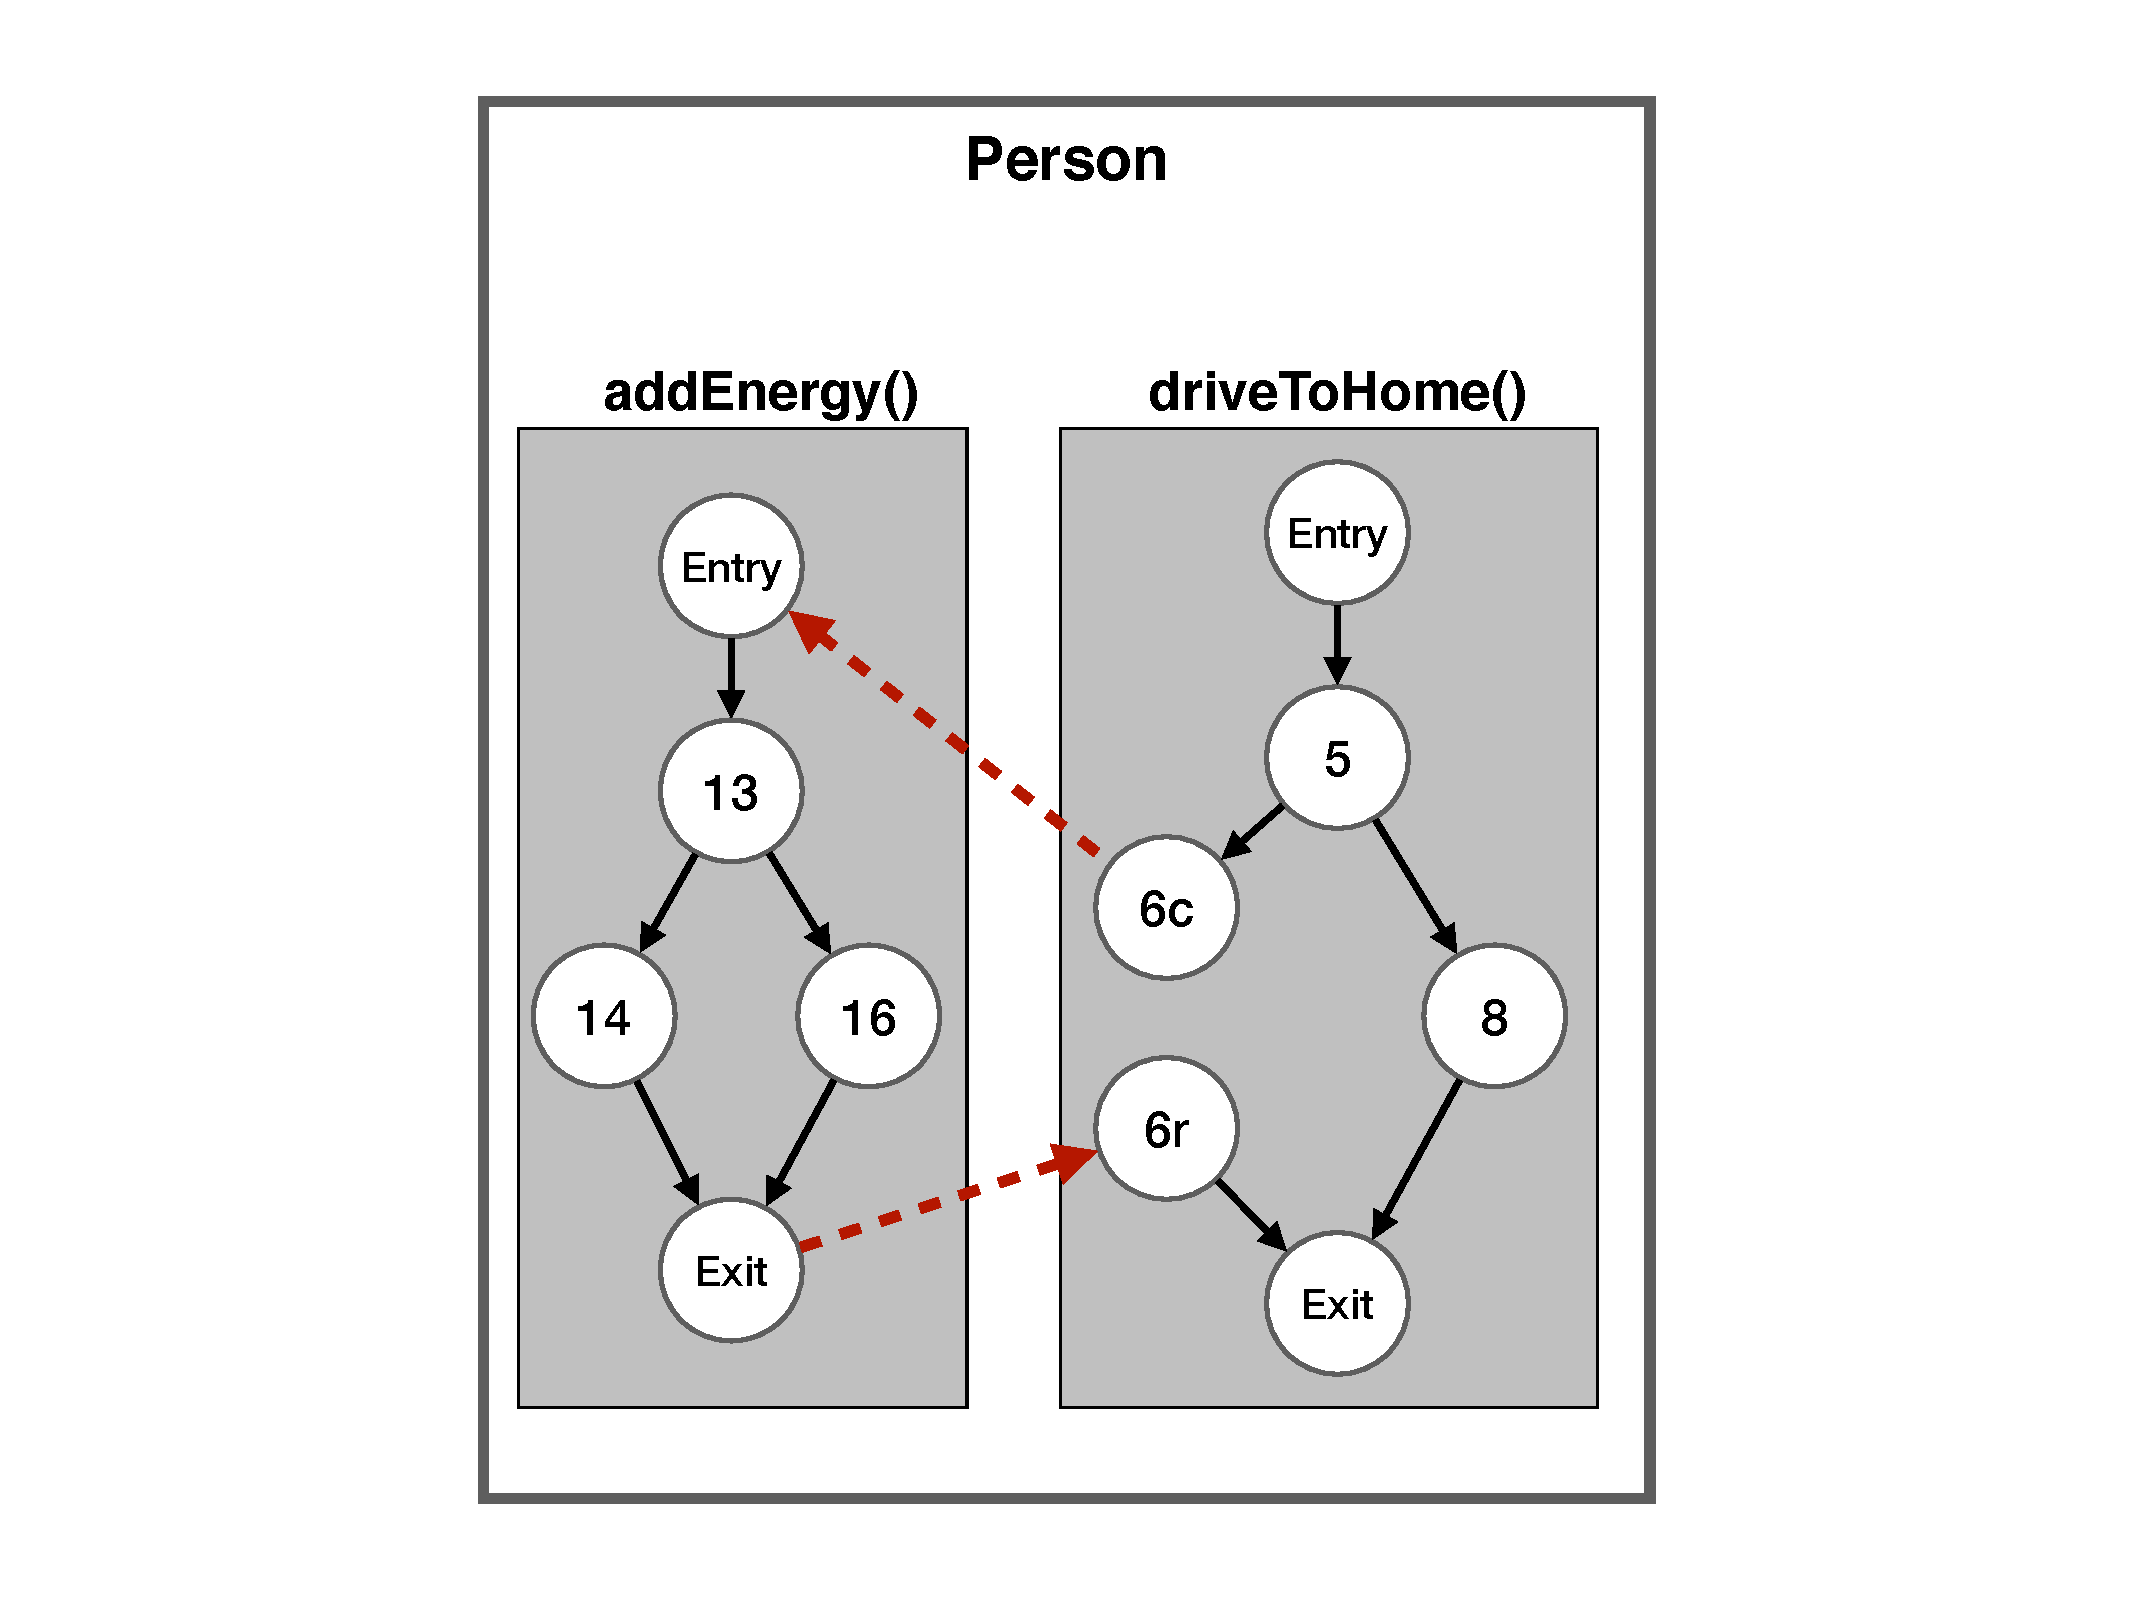
\includegraphics[width=0.85\linewidth]{figs/CCFG_new}
	\caption{Class-level CFG for class \texttt{Person}}
  \label{fig:CCFG}
\end{figure}


Many structural-based approaches combine two common heuristics to reach a high branch and statement coverage in unit-level testing. These two heuristics  are \textit{approach level} and \textit{branch distance}.
The \textit{branch distance} measures (based on a set of rules) the distance to \textit{satisfying} (true branch) and the distance to \textit{not satisfying} (false branch) a particular branching node in the program.
The \textit{approach level} measures the distance between the execution path and a target node in a CFG. To describe how this heuristic measures this distance, we 
rely on the concepts of \textbf{post-dominance} and \textbf{control dependency}~\cite{Allen:1970:CFA:800028.808479}. 

%
As an example, in Figure \ref{fig:CCFG}, \textit{node 8} is control dependent on \textit{node 5} and \textit{node 8} post-dominates edge $\langle 5,8\rangle$. %, but it does not post-dominate $node 5$ itself ($node 5$ can reach the exit point through $node 6$). 
The \textit{approach level} is the minimum number of control dependencies between a target node and an executed path by a test case. 


\subsection{Automated Crash Reproduction}

Crash reproduction approaches can be divided into three categories, based on the kind of data used for crash reproduction: \emph{record-replay approaches} record data from the running program; \emph{post-failure approaches} collect data from the crash, like memory dump; and \emph{stack-trace based post-failure} use only the stack trace produced by the crash. We briefly describe each category hereafter.

\paragraph{Record-replay approaches.}

These approaches record the program runtime data and use them during crash reproduction. The main limitation is the availability of the required data. Monitoring software execution may violate privacy by collecting sensitive data, the monitoring process can be an expensive task for the large scale software, and may induce a significant overhead \cite{Chen2015, Nayrolles2017, Rossler2013}.
%
Tools like \textrm{ReCrash} \cite{Artzi2008}, \textrm{ADDA} \cite{Clause2007}, \textrm{Bugnet} \cite{Narayanasamy2005}, \textrm{jRapture} \cite{Steven2000}, \textrm{MoTiF} \cite{Gomez2016}, \textrm{Chronicler} \cite{Bell2013}, and \textrm{SymCrash} \cite{Cao2014} fall in this category.


\paragraph{Post-failure approaches.}

Techniques from this category use the software data collected directly after the occurrence of a failure. For instance, \textrm{RECORE} \cite{Rossler2013} applies a search-based approach to reproduce a crash by using the stack trace and a core dump, produced by the system when the crash happened, to guide the search.
% Instead, \evocrash only considers the stack trace (usually provided when a bug is reported in an issue tracker) and a distance, similar to the one described by Rossler \etal \cite{Rossler2013}, to guide the search.

Although these tools limit the quantity of monitored and recorded data, the availability of such data still represents a challenge. 
Yu \etal \cite{YZW17descry} addressed this issue for system-level concurrency failure reproduction by introducing \textrm{DESCRY}. 
This approach only uses the default execution logs and applies both static and dynamic analysis combined with symbolic execution to generate the input data and interleaving schedule. 
However, even this approach suffers from two limitations: 
\begin{inparaenum}[(i)]
\item since this tool relies on symbolic execution, applying it on the large and complex projects leads to path explosion;
\item the performance of this tool is strongly linked to the quality of the software log.
\end{inparaenum}
%
Other \textit{post-failure approach} inlcude: Weeratunge \etal \cite{Weeratunge2010}, Leitner \etal \cite{Leitner2007, Leitner2009}, and Kifetew \etal \cite{Kifetew2013, Kifetew2014}.

\paragraph{Stack-trace based post-failure.}

Recent studies in crash reproduction \cite{BPT17concrash,soltani2017,Nayrolles2017,Xuan2015,Chen2015} focuses on utilizing data only from a given crash stack trace to enhance the practical application. 
%
Table~\ref{tab:ant49755} illustrates an example of a crash stack trace from Apache Ant\footnote{ANT-49755: \url{https://bz.apache.org/bugzilla/show_bug.cgi?id=49755} } ~\cite{ant} which is comprised of a crash type (\texttt{java.lang.Null\-Pointer\-Exception}) and a stack of frames pointing to all method calls that were involved in the execution when the crash happened.
From a crash stack frame, we can retrieve information about: the crashing method, the line number in the method where the crash happened, and the fully qualifying name of the class where the crashing method is declared.

\begin{table*}[t]
\centering
\caption{The crash stack trace for Apache Ant-49755.}
\label{tab:ant49755}
\begin{tabular}{c|l}
\multicolumn{2}{l}{java.lang.\textbf{NullPointerException}:}\\
\hline
\textbf{Level} & \textbf{Frame} \\
\hline
1 & \textbf{at} org.apache.tools.ant.util.FileUtils.\textbf{createTempFile}(FileUtils.java:\textbf{888})\\
2 & \textbf{at} org.apache.tools.ant.taskdefs.TempFile.\textbf{execute}(TempFile.java:\textbf{158})\\
3 & \textbf{at} org.apache.tools.ant.UnknownElement.\textbf{execute}(UnknownElement.java:\textbf{291}) \\
\end{tabular}
\end{table*}

The state of the research in crash reproduction \cite{Zamfir2010, jin2012bugredux, BPT17concrash, soltani2017, Nayrolles2017, Xuan2015, Chen2015} aims at generating test code that, once executed, produces a stack trace that is as similar to the original one as possible. They, however, differ in their means to achieve this task. 

\textrm{ESD} \cite{Zamfir2010} uses forward symbolic execution and static analysis to reach reproduction. This tool focuses more on concurrency and memory safety bugs.
Similarly, \textrm{BugRedux} \cite{jin2012bugredux} uses forward symbolic execution. \textrm{BugRedux} is a crash reproduction tool for C programs.

Since these two tools rely on forward symbolic execution, they can be applied only on medium-size applications. Also, as illustrated by Braione \etal \cite{braione2017tardis}, symbolic execution test generation approaches face limitations when generating complex input data structures.
To address these limitations, \textrm{STAR} \cite{Chen2015} applies optimized backward symbolic execution and uses a novel technique for method sequence composition to generate a unit test that satisfies the computed preconditions, and eventually reproduces the target crash. 
However, as reported by Chen \etal \cite{Chen2015}, \textrm{STAR} still suffers from the path explosion stemming from utilizing symbolic execution. 
It only supports 3 types of exceptions: explicitly thrown exceptions, \texttt{NullPointerException}, and \texttt{ArrayIndexOutOfBoundsException}.  

\textrm{JCHARMING} \cite{Nayrolles2017} applies model checking to reproduce the reported bugs. To prevent state explosion in the model, it utilizes program slicing.
Since \textrm{JCHARMING} can be applied to any frame from a given crash stack trace, the approach can reproduce any fraction of the target crash stack trace. 

\textrm{MuCrash} \cite{Xuan2015} is based on exploiting existing test cases written by developers and mutating them until they trigger the target crash.
Test case mutation in \textrm{MuCrash} is directed by selecting tests for the classes included in the target crash stack trace. 

Finally, \textrm{Concrash} \cite{BPT17concrash} focuses on reproducing \textit{concurrency} failures that violate thread-safety of a class.
\textrm{Concrash} iteratively generates test code and looks for a thread interleaving that triggers a concurrency crash.
In order to steer the test generation process and avoid expensive computations, \textrm{Concrash} applies the pruning strategies to avoid redundant and irrelevant test code. In contrast with other crash reproduction techniques, \textrm{Concrash} only reproduces the minority of the crashes in the issue tracking systems. As reported by Yuan \etal \cite{Yuan2014}, inter-leaving crashes cause only 10\% of failures in the distributed data-intensive systems. Besides, Coelho \etal \cite{Coelho2015} state that this number is even lower in the Android applications (2.9\%).

\subsection{Search-based crash reproduction with \evocrash}

Search-based algorithms have been increasingly used for software engineering problems since they are shown to suite complex, non-linear problems, with multiple optimization objectives that may conflict or competing~\cite{harman12trends}.
\evocrash \cite{soltani2017, Soltani2018a} is a search-based approach to crash reproduction, which applies a \textit{guided genetic algorithm} to search for a unit test that reproduces the target crash.

\evocrash takes as input a stack trace with one of its frames set as the \emph{target frame}. 
The target frame is composed of 
(i) \emph{target class}, the class to which the exception has been propagated;
(ii) \texttt{target method}, the method in that class; and 
(iii) \emph{target line}, the line in that method where the exception has been propagated. 
It then seeks to generate a unit test that replicates the given stack trace from the target frame (at level $n$) to the deepest frame (at level 1). 
For instance, if we pass the stack trace in Table \ref{tab:ant49755} as the given trace and indicate the second frame as the target frame (level 2), the output of \evocrash will be a unit test for the class \texttt{TempFile} which replicates the first two frames of the given stack trace with the same type of the exception (\texttt{NullPointerException}).

\subsubsection{Guided genetic algorithm}

The search process in \evocrash begins by randomly generating unit tests for the target frame.
In this phase, called \emph{guided initialization}, the target method corresponding to the selected frame (i.e., the \emph{failing method} to which the exception is propagated) is injected in every randomly generated unit test.
During subsequent phases of the search, \emph{guided crossover} and \emph{guided mutation}, standard evolutionary operations are applied to the unit tests.
However, applying these operations involves the risk of losing the injected failing method.
Therefore, the algorithm ensures that only unit tests with the injected failing method call remain in the evolution loop. 
If the generated test by crossover does not contain the failing method, the algorithm replaces it with one of its parents. 
Also, if the resulting test does not contain the failing method after a mutation, the algorithm redoes the mutation until the failing method is added to the test again.
The search process continues until either the search budget is over or a crash reproducing test case is found.

To evaluate the generated tests, \evocrash applies the following weighted sum fitness function \cite{Soltani2018a} to a generated test $t$:
%
\rowcolors{1}{}{}
\begin{equation} \label{eq:fitnessfunction}
f(t) = 
\left\{
  \begin{array}{lcr}
    3 \times d_{s}(t) + 2 \times max(d_{except}) + max(d_{trace})   && \textit{if the line is not reached}\\
    3 \times min(d_{s}) + 2 \times d_{except}(t) + max(d_{trace})   && \textit{if the line is reached}\\
    3 \times min(d_{s}) + 2 \times min(d_{except}) + d_{trace}(t)   && \textit{if the exception is thrown}
  \end{array}
\right.
\end{equation}
\rowcolors{1}{}{gray!15}
%
Where:
%
\begin{itemize}
\item $d_{s} \in [0,1]$ indicates the distance between the execution of $t$ and the target statement $s$ located at the target line. 
This distance is computed using the \textit{approach level}, measuring the minimum number of control dependencies between the path of the code executed by $t$ and $s$, and normalized \textit{branch distance}, scoring how close $t$ is to satisfying the branch condition for the branch on which$s$ is directly control dependent \cite{McMinn2004}. 
If the target line is reached by the test case, $d_{l}(t)$ equals to $0.0$;
%
\item $d_{except}(t) \in \{0,1\}$ indicates if the target exception is thrown ($d_{e} = 0$) or not ($d_{e} = 1$);
%
\item $d_{trace}(t) \in [0,1]$ indicates the similarity of the input stack trace and the one generated by $t$ by looking at class names, methods names and line numbers;
%
\item $max(\cdot)$ denotes the maximum possible value for the function.
\end{itemize}
%
Since the stack trace similarity is relevant only if the expected exception is thrown by $t$, and the check whether the expected exception is thrown or not is relevant only if the target line where the exception propagates is reached, $d_{except}$ and $d_{trace}$) are computed only upon the satisfaction of two \emph{constraints}: the target exception has to be thrown in the target line $s$ and the stack trace similarity should be computed only if the target exception is actually thrown. 

Unlike other stack trace similarity measures (e.g., \cite{Rossler2013}), Soltani \etal \cite{Soltani2018a} does not require two stack traces to share the same common prefix to avoid rejecting stack traces where the difference is only in one intermediate frame. Instead, for each frame, $d_{trace}(t)$ looks at the closest frame and compute a distance value. Formally, for an original stack trace $S*$ and a test case $t$ producing a stack trace $S$, $d_{trace}(t)$ is defined as follows:
%
\rowcolors{1}{}{}
\begin{equation}
d_{trace}(t) = \varphi \left( \sum_{f* \in S*} min \left\lbrace \mathit{diff}(f*, f) : f \in S \right\rbrace \right)
\end{equation}
\rowcolors{1}{}{gray!15}
%
Where $\varphi (x) = x / (x+1)$ is a normalization function \cite{McMinn2004} and $\mathit{diff}(f*, f)$ measures the difference between two frames as follows: 
%
\rowcolors{1}{}{}
\begin{equation}
\mathit{diff}(f*, f) = 
\left\{
  \begin{array}{lcr}
    3 && \textit{if the classes are different}\\
    2  && \textit{if the classes are equal but the methods are different}\\
     \varphi \left( \vert l* - l \vert \right)   && \textit{otherwise}
  \end{array}
\right.
\end{equation}
\rowcolors{1}{}{gray!15}
%
Where $l$ (resp. $l*$) is the line number of the frame $f$ (resp. $f*$).

Each of the three components if the fitness function defined in Equation \ref{eq:fitnessfunction} ranges from $0.0$ to $1.0$, the overall fitness value for a given test case ranges from $0.0$ (crash is fully reproduced) to $6.0$ (no test was generated), depending on the conditions it satisfies. 

\subsubsection{Comparison with the state-of-the-art}

\paragraph{Other crash reproduction techniques.}
%
A recent study \etal \cite{soltani2017, Soltani2018a} compared \evocrash with other stack-trace based crash reproduction approaches: \textsc{STAR} \cite{Chen2015}, \textsc{JCHARMING} \cite{Nayrolles2017}, and \textsc{MuCrash} \cite{Xuan2015}.
According to their results, \evocrash outperforms other tools.
% Only one crash (ACC-104) could be replicated by \textsc{STAR} and \textsc{MuCrash} but not by \evocrash. 
% After manual analysis, Soltani \etal identified an ``\textit{inheritance problem}'': \evocrash instantiates an object from the wrong subclass during the search process. 
% This issue has been confirmed in our evaluation and identified as a challenge for crash reproduction and search-based software testing.
% Unfortunately, as explained by Soltani \etal \cite{soltani2017, Soltani2018a}, other crash reproduction tools are not publicly available, and the reported comparisons in these studies are performed based on results published in \cite{Chen2015, Nayrolles2017, Xuan2015}. 

\paragraph{\evosuite{}.}
%
Also, it has been shown that \evocrash outperforms \evosuite, with exception coverage as the primary objective \cite{Soltani2018a}. 
Out of 52 crashes, \evocrash replicated 46 crashes(85\%), while \evosuite replicated only 18 crashes (33\%). 
All the crashes reproduces by \evosuite could also be reproduced by \evocrash on average 170\% faster, and with a higher reproduction rate. 

\subsubsection{Usefulness for debugging}

When reproducing a stack trace with \evocrash, there is no guarantee that the generated test reproduces completely the conditions in which the crash happened in the first place. Besides the random nature of search-based approaches, test cases are generated at the unit level, while crashes usually happen at the system level. However, rather than reproducing the exact same conditions of the crash, the goal of crash reproduction is to help developers fix the underlying bug.

Chen \etal \cite{Chen2015} introduced a usefulness criterion for the crash reproduction approaches. 
According to this criterion, a crash reproducing test is useful to the developers if it covers the buggy frame: i.e., if the target frame for which the reproduction is successful is higher than the frame that points to the buggy method.
Soltani \etal \cite{Soltani2018a} refined that criterion trough a controlled experiment with 35 master students in computer science and two crashes to assess the degree to which the tests generated by \evocrash helps to debug code. 
Their results indicate that the reproducing tests generated by \evocrash help the participants to fix the bugs more often, although not significantly, and significantly faster. 
They confirmed the usefulness criterion defined by the Chen \etal \cite{Chen2015} but also found evidence that test cases categorized as not useful can still help developers fix the bug.

\section{Challenges In Search-based Crash Reproduction And Test Generation}
Since the search-based crash reproduction approaches are evaluated by a limited number of crashes, the limits and challenges of these techniques remained largely unrecognized.
In this thesis, we first identify search-based crash reproduction challenges. Hence, we empirically evaluate search-based crash reproduction by a new Java crash benchmark called \jcrashpack and identify the challenges by performing an extensive manual analysis. Some of the identified challenges are dedicated only to the crash reproduction problem, but some other challenges are general search-based test generation issues.

After identifying the challenges, we intend to address them by introducing novel solutions to improve the effectiveness and efficiency of the crash reproduction search process. For this goal, we investigate the application of contextual information collected from different sources such as source code, manually-written test cases. While some identified challenges in search-based crash reproduction are due to the existing general search-based test generation limitations, we go beyond crash reproduction and introduce new search-based techniques to cover other specific software behaviors.

\section{Research Goals \& Questions}
This thesis seeks to understand the challenges in search-based crash reproduction and test case generation and utilizes the existing information in different sources such as source code and manually-written test cases to address the identified challenges.
Hence, to present indications towards this thesis, we seek to answer the following research questions:

Since our initial goal is improving the effectiveness and efficiency of the search-based crash reproduction, first, we need to understand its challenges. Hence, the first research question tries to address this goal.
\begin{framed}
\quad\textbf{RQ$_1$: } \textit{What are the challenges in search-based crash reproduction?}
\end{framed}

After identifying the challenges, we study novel ways to tackle them by enhancing the search process from different aspects. This enhancement is done by utilizing the contextual information collected from source code and existing tests. The second research question investigates the new techniques addressing the detected challenges using the observed contextual information.


\begin{framed}
    
    \textbf{RQ$_2$: } \textit{Based on the identified challenges, how can we leverage the existing knowledge, carved from information sources, to steer the crash reproduction search process?}

\end{framed}

Since some of the detected challenges in search-based crash reproduction are observable in other search-based test generation techniques, the observed contextual information can guide the search process to generate tests for other criteria, as well. Hence, the last question concentrates on novel search-based techniques for testing in two levels of unit testing and class integration testing.

\begin{framed}
    \textbf{RQ$_3$: } \textit{How can we leverage the existing knowledge, carved from information sources, to design search-based test generation approaches for unit and class integration testing?}
\end{framed}

This thesis answers $RQ_3$ by (i) introducing a whole new search-algorithm for class integration testing using the collected information about the method calls from one class (\textit{caller class}) to the other one (\textit{callee class}), and (ii) introducing a new search objective for search-based unit testing considering the common and uncommon execution paths in the class under test.

After answering these research questions, we will be able to understand the challenges in search-based software test generation better. Besides, we can confirm that (i) automated test generation for specific software behaviors can cover, and reveal, faults that are not detectable by other search-based test generation techniques, using only the classical structural coverage search objectives; and (ii) using other contextual information collected from various sources (such as source code, existing test cases, and execution logs) guides the search process to achieve higher fault detection.





\section{Research Outline}

This section briefly presents the various chapters in this thesis.
Table \ref{tab:chaptersvsRQs} outlines the connections between each defined research question and chapters in this thesis.


\begin{table}[!t]
\caption{Connection of chapters with research questions}
\label{tab:chaptersvsRQs}
\begin{tabular}{|p{0.8\textwidth}||c|}
\textbf{Research Question} & \textbf{Chapters}\\
\hline
\hline
$RQ_1$: What are the challenges in search-based crash reproduction? & 2\\
$RQ_2$: Based on the identified challenges, how can we leverage the existing knowledge, carved from information sources, to steer the crash reproduction search process? & 3 to 5\\
$RQ_3$: How can we leverage the existing knowledge, carved from information sources, to design search-based test generation approaches for unit and class integration testing? & 6 \& 7\\
\hline
\end{tabular}
\end{table}


\paragraph{Chapter 2:}%JCrashPack paper (adressing $RQ_1$)
Crash reproduction approaches help developers during debugging by generating a test case that reproduces a given crash. 
Several solutions have been proposed to automate this task.
However, the proposed solutions have been evaluated on a limited number of projects, making comparison difficult.
In this chapter, we enhance this line of research by proposing \crashpack, an extensible benchmark for Java crash reproduction, together with \exrunner, a tool to simply and systematically run evaluations.
\crashpack contains 200 stack traces from various Java projects, including industrial open source ones, on which we run an extensive evaluation of \evocrash, the state-of-the-art approach for search-based crash reproduction.
Our results include a detailed manual analysis of \evocrash outputs, from which we derive 14 current challenges for crash reproduction. 
Finally, based on those challenges, we discuss future research directions for search-based crash reproduction for Java.

\paragraph{Chapter 3:}%Model seeding (adressing $RQ_2$)
According to the results of Chapter 2, one of the fundamental challenges of search-based crash reproduction is creating objects needed to trigger the crash. One way to overcome this limitation is seeding: using information about the application during the search process. With seeding, the existing usages of classes can be used in the search process to produce realistic sequences of method calls which create the required objects. In this chapter, we introduce behavioral model seeding: a new seeding method which learns class usages from both the system under test and existing test cases.  Learned usages are then synthesized in a behavioral model (state machine). Then, this model serves to guide the evolutionary process. To assess behavioral model-seeding, we evaluate it against test-seeding (the state-of-the-art technique for seeding realistic objects) and no-seeding (without seeding any class usage). 
Our results indicate that behavioral model-seeding outperforms both test seeding and no-seeding by a minimum of 6\% without any notable negative impact on efficiency.

%\textbf{Chapter ?: } Multi-objectivization paper (adressing $RQ_2$)

\paragraph{Chapter 4:}% MOHO paper (adressing $RQ_2$)
The state-of-the-art search-based crash reproduction approaches use a single fitness function called \CrashFunction to guide the search process toward reproducing a target crash. Despite the reported achievements, these approaches do not always successfully reproduce some crashes due to a lack of test diversity (premature convergence). In this study, we introduce a new approach, called \moho, that addresses this issue via multi-objectivization. In particular, we introduce two new Helper-Objectives for crash reproduction, namely \textit{test length} (to minimize) and \textit{method sequence diversity} (to maximize), in addition to \CrashFunction.
We assessed \moho using five multi-objective evolutionary algorithms (NSGA-II, SPEA2, PESA-II, MOEA/D, FEMO) on crashes selected from \crashpack. Our results indicate that SPEA2 is the best-performing multi-objective algorithm for \moho.
We evaluated this best-performing algorithm for \moho against the state-of-the-art: single-objective approach (\SGGA) and decomposition-based multi-objectivization approach (\decomposition). Our results show that \moho reproduces five crashes that cannot be reproduced by the current state-of-the-art. Besides, \moho improves the effectiveness (+10\% and +8\% in reproduction ratio) and the efficiency in 34.6\% and 36\% of crashes (i.e., significantly lower running time) compared to  \SGGA and \decomposition, respectively. For some crashes, the improvements are very large, being up to +93.3\% for reproduction ratio and -92\% for the required running time. 

\paragraph{Chapter 5:}%Basic Block Coverage paper (adressing $RQ_2$)
Search-based crash reproduction approaches rely on the \emph{approach level} and \emph{branch distance} heuristics to guide the search process and generate test cases covering the lines, which appeared in the given stack trace.
Despite the positive results achieved by these two heuristics, they only use the information related to the coverage of explicit branches (\eg indicated by conditional and loop statements), but ignore potential implicit branchings within basic blocks of code. 
If such implicit branching happens at runtime (\eg if an exception is thrown in a branchless-method), the existing fitness functions cannot guide the search process. 
To address this issue, we introduce a new secondary objective, called Basic Block Coverage (\bbc), which takes into account the coverage level of relevant basic blocks in the control flow graph. We evaluated the impact of \bbc on \emph{search-based crash reproduction} because the implicit branches commonly occur when trying to reproduce a crash, and the search process needs to cover only a few basic blocks (\ie blocks that are executed before crash happening). We combined \bbc with existing fitness functions (namely \integ and \WS) and ran our evaluation on \crashpack crashes.
Our results show that \bbc, in combination with \integ and \WS, reproduces 6 and 1 new crashes, respectively.
\bbc significantly decreases the time required to reproduce 26.6\% and 13.7\% of the crashes using \integ and \WS, respectively. For these crashes, \bbc reduces the consumed time by 44.3\% (for \integ) and 40.6\% (for \WS) on average.

\paragraph{Chapter 6:}%CLING paper (adressing $RQ_3$)
Search-based approaches have been used in the literature to automate the process of creating unit test cases. However, related work has shown that generated unit-tests with high code coverage could be ineffective, i.e., they may not detect all faults or kill all injected mutants. 
In this chapter, we propose \cling, an integration-level test case generation approach that exploits how a pair of classes, the caller and the callee, interact with each other through method calls. In particular, \cling generates integration-level test cases that maximize the Coupled Branches Criterion (CBC). CBC is a novel integration-level coverage criterion, measuring the degree to which a test suite exercises the interactions between a caller and its callee classes. 
We implemented \cling and evaluated the approach on 140 pairs of classes from five different open-source Java projects. Our results show that (1) \cling generates test suites with high CBC coverage; (2) such generated suites can kill 
on average 7.7\% (with a maximum of 50\%) of mutants that are not detected by tests generated at the unit level; (3) \cling can detect integration faults (32 for our subject systems) that remain undetected when using automatically generated unit-level test suites. 

\paragraph{Chapter 7:}%Common behavior (adressing $RQ_3$)
Various search-based test generation techniques have been proposed to automate the generation of unit tests fulfilling different criteria (\eg line coverage, branch coverage, mutation score, \etc). Despite several advances made over the years, search-based unit test generation still suffers from a lack of guidance due to the limited amount of information available in the source code that, for instance, hampers the generation of complex objects. Previous studies introduced many strategies to address this issue, \eg dynamic symbolic execution or seeding, but do not take the internal execution of the methods into account.  
This chapter introduces a novel secondary objective called \emph{commonality score}, measuring how close the execution path of a test case is from reproducing a \emph{common} or \emph{uncommon} execution pattern observed during the operation of the software.
To assess the commonality score, we implemented it in \evosuite and evaluated its application on 150 classes from \jabref, open-source software for managing bibliographic references. 
Our results are mixed. Our approach leads to test cases that indeed follow \emph{common} or \emph{uncommon} execution patterns. However, if the commonality score can have a positive impact on the structural coverage and mutation score of the generated test suites, it can also be detrimental in some cases. 

\paragraph{Chapter 8:} 
Finally, we summarize our findings and conclusions in this thesis. This chapter also elaborates on the potential future work that can, first, improve the search-based crash reproduction, and second, investigate novel search-based algorithms for covering other software specific behaviors that can be interesting for developers.


\section{Research Methodology}

This thesis answers the aforementioned research questions by following an approach based on design science \cite{Hevner2004}.
The design science paradigm contains two iterative phases: \textbf{Build} and \textbf{Evaluation}. The former phase concentrates on developing a purposeful artifact to solve an unsolved problem (here, search-based test generation techniques for specific behaviors such as crash reproduction and class integrations). The latter phase evaluates the designed artifact.
The \textit{Evaluation} phase reveals the limitations and challenges in the built artifact, and thereby, the weaknesses can be identified and resolved in the next phase of the \textit{Build} process. This iteration usually continues multiple times, and in each iteration, one (or more) novel techniques are introduced (to improve the existing artifact) and be assessed by the \textit{Evaluation} process. Also, both \textit{Build} and \textit{Evaluation} evolve in this process according to the new findings. 

In this thesis, we define a framework for search-based test case generation for crash reproduction. This framework includes a benchmark for crash reproduction approaches containing real-world and non-trivial crashes, an extensible platform for search-based crash reproducing test case generation, and accompanying guidelines for efficient usage of the platform in an industrial setting. This framework applies the existing search-based crash reproduction approach to real-world crashes and identifies the challenges (to answer $RQ_1$). We then improve the crash reproduction approach by addressing the identified challenges (to answer $RQ_2$). Finally, we go beyond search-based crash reproduction and introduce a novel approach for generating tests to cover other specific behaviors (\eg class integration testing). Accordingly, we extend the evaluation process to assess the new artifacts, as well (to address $RQ_3$).



\section{Origins Of The Chapters}
All chapters of this thesis (except Chapter 7, which is currently under review) have been published in peer-reviewed journals and conferences. 
Hence, some chapters contain a dedicated background, related work, and conclusion section. 
This section lists the origin of each chapter.

\begin{itemize}
    \item \textit{Chapter 2} was published in the paper "A benchmark-based evaluation of search-based crash reproduction" in Empirical Software Engineering Journal (EMSE) 2020.
    \item \textit{Chapter 3} was published in the paper "Search‐based crash reproduction using behavioural model seeding" in Journal of Software: Testing, Validation, and Reliability (STVR) 2020.
    \item \textit{Chapter 4} was published in the paper " Good Things Come In Threes: Improving Search-based Crash Reproduction With Helper Objectives" at International Conference on Automated Software Engineering (ASE) 2020.
    \item \textit{Chapter 5} was published in the paper "It is not Only About Control Dependent Nodes: Basic Block Coverage for Search-Based Crash Reproduction" at Symposium on Search-Based Software Engineering (SSBSE) 2020.
    \item \textit{Chapter 6} was published is a paper called "Generating Class-Level Integration Tests Using Call Site Information", which is currently under revision in Transactions on Software Engineering journal (TSE).
    \item \textit{Chapter 7} was published in the paper "Commonality-Driven Unit Test Generation" at Symposium on Search-Based Software Engineering (SSBSE) 2020.
  \end{itemize}

\section{Open Science}
\label{sec:intro:open}
Open science is the “movement to make scientific research, data and dissemination accessible to all levels of an inquiring society” \cite{Open_science}. All of the implementations used in our studies are available via GitHub. Also, replication packages of all of our studies, presented in this thesis, are openly available in Zenodo. These replication packages contain the list of subjects used in each study, a Docker-based infrastructure to rerun all of the experiments, and all test cases generated by each of the search-based approaches.

Table \ref{tab:replicationpackages} shows the replication package of each chapter in this thesis.

\begin{table}[!t]
    \begin{center}
        
    \footnotesize
    \caption{Connection of chapters with replication packages}
    \label{tab:replicationpackages}
    \begin{tabular}{|c||c|c|}
    \textbf{Chapter} & \textbf{Replication package} & \textbf{Zenodo DOI}\\
    \hline
    \hline
    2 & \cite{zenodoJCrashPack}& 10.5281/zenodo.3766689 \\
    3 & \cite{pouria_derakhshanfar_2019_3673916}& 10.5281/zenodo.3673916 \\
    4 & \cite{zenodoRP}& 10.5281/zenodo.3979097 \\
    5 & \cite{derakhshanfar_pouria_2020_3953519}& 10.5281/zenodo.3953519\\
    6 & \url{https://github.com/STAMP-project/Cling-application}& - \\
    7 & \cite{evers_bjorn_2020_3894711}& 10.5281/zenodo.3894711\\
    \hline
    \end{tabular}
\end{center}
    \end{table}

\subsection{Open-source Search-based Test Case Generation Implementations}
\subsubsection{Search-based crash reproduction (\botsing)}
In this thesis, we present \botsing\footnote{\url{https://github.com/STAMP-project/botsing}}: an open-source, extendable search-based crash reproduction framework. \botsing implements search-based crash reproduction approaches introduced in previous studies~\cite{Rossler2013, Soltani2018a, Soltani2018b}. The tool takes as input a stack trace and software under test. Then, it starts a single-objective or multi-objective search process to generate a test reproducing the crash.

\botsing has been designed as an extendable framework for implementing new features and search algorithms for crash reproduction. For example, in Chapter 3 we perform a study on the impact of various \emph{seeding} strategies on crash reproduction, we have implemented multiple seeding strategies in \botsing.

From an industrial perspective, \botsing is used by our partners in the STAMP project.\footnote{Available at \url{http://stamp-project.eu/}}
They confirmed the relevance of \botsing for debugging and fixing application crashes~\cite{D57}.
The feedback ---as well as the crash reproducing test cases--- from our partners using \botsing are openly available in the STAMP GitHub repository.\footnote{Available at \url{https://github.com/STAMP-project/botsing-usecases-output}.}

\subsubsection{Search-based test generation for class integration (\cling)}
Chapter 6 addresses the $RQ_3$ by introducing a novel search-based technique to test the integration between two classes their call-sites information. We have implemented this approach as an open-source tool called \cling\footnote{\url{https://github.com/STAMP-project/botsing/tree/master/cling}}. This tool gets \emph{application's bytecode} and two classes in the application (\emph{caller class} and \emph{callee class}) and produces a test suite that covers the various interactions between these two classes.

\subsubsection{Common/uncommon execution patterns test generation in unit testing}
In Chapter 7, we implement novel secondary objectives considering the common/uncommon execution patterns in \evosuite, which is a well-known open-source unit test generation framework.

\subsection{Open-source Evaluation Infrustructures}

\subsubsection{Assessing crash reproduction}
To evaluate the different search-based crash reproduction techniques, we created \jcrashpack, an open-source crash benchmark, which contains 200 non trivial Java crashes collected from seven open-source projects: \textit{Closure compiler}, \textit{Apache commons-lang}, \textit{Apache commons-math}, \textit{Mockito}, \textit{Joda-Time}, \textit{XWiki}, and \textit{ElasticSearch}.
Moreover, to ease benchmarking using \crashpack, we developed a bash-based execution runner, openly available on GitHub.\footnote{\url{https://github.com/STAMP-project/ExRunner-bash}} This experiment runner (called \exrunner) runs different instances of a crash reproduction tool (here, \botsing) in parallel processes and collects relevant information about the execution in a CSV file. These collected data helps to identify the search-based crash reproduction benchmark.

\subsubsection{Assessing class integration} 
To assess \cling against the state-of-the-art, we used subjects from five Java projects, namely \textit{Closure compiler}, \textit{Apache commons-lang}, \textit{Apache commons-math}, \textit{Mockito}, and \textit{Joda-Time}. These 
projects have been used in prior studies to assess the coverage and the effectiveness of unit-level test case generation \cite{ma2015grt, Panichella2018, just2014defects4j, Shamshiri2016}, program repair \cite{smith2015cure, martinez2016astor}, fault localization \cite{pearson2017evaluating, b2016learning}, and regression testing \cite{noor2015similarity, lu2016does}.

Moreover, we have implemented another open-source runner \footnote{\url{https://github.com/STAMP-project/Cling-application}} (similar to \exrunner). This runner collects more information about the test suites generated by different approaches: \textit{branch coverage} and mutatio score measured by PIT\footnote{http://pitest.org}, which is a state-of-the-art mutation testing tool for Java code, to mutate the callee classes.

\subsubsection{Assessing common/uncommon execution patterns test generation} 

To assess our common/uncommon execution patterns search objective, we choose \jabref (46 KLOC), an open-source Java bibliography reference manager with a graphical user interface working with BibTex files. We instrumented \jabref using Spoon~\cite{pawlak:hal-01169705} to monitor the execution paths while users are using it. We sampled 150 classes from this project for our evaluation.

Since we want to measure the strong mutation score of test suites generated by \evosuite + our novel secondary objectives against regular \evosuite, we use the same open-source infrastructure as the one we used to assess \cling.

% In this thesis \cite{Derakhshanfar2020}, you can reference pictures~\Cref{fig:devmodel} using Cleverref and circles \circled{5}.

% \begin{figure}[htb]
% 	\centering
% 	\includegraphics[width=0.65\columnwidth]{development_model_without_papers}
% 	\caption{The stages of the FDD model and their relationship to other
%           Software Engineering concepts.}
% 	\label{fig:devmodel}
% \end{figure}

% We also have lists:

% \begin{enumerate}
%   \item Static Analysis~\circled{3} examines program artifacts or
%     their source code without executing them~\cite{wichmann1995industrial}, while
%  \item Dynamic Analysis~\circled{4} relies on information gathered from their
%    execution~\cite{cornelissen2009systematic}.
% \end{enumerate}

% Or boxes:

% \begin{framed}
% This thesis is concerned with the empirical assessment of the state of the art of how developers
% drive software development with the help of feedback loops.
% \end{framed}

% Or code:
% \begin{lstlisting}[caption={\textsc{TrinityCore}},label={lst:e1}]
%  x += other.x;
%  y += other.y;
%  z += other.y;
% \end{lstlisting}




% Long: \acrlong{fdd}

% Short: \acrshort{fdd}

% Full: \acrfull{fdd}
